\documentclass[12pt,letterpaper]{article}
\usepackage{graphicx,textcomp}
\usepackage{natbib}
\usepackage{setspace}
\usepackage{fullpage}
\usepackage{color}
\usepackage[reqno]{amsmath}
\usepackage{amsthm}
\usepackage{fancyvrb}
\usepackage{amssymb,enumerate}
\usepackage[all]{xy}
\usepackage{endnotes}
\usepackage{lscape}
\newtheorem{com}{Comment}
\usepackage{float}
\usepackage{hyperref}
\newtheorem{lem} {Lemma}
\newtheorem{prop}{Proposition}
\newtheorem{thm}{Theorem}
\newtheorem{defn}{Definition}
\newtheorem{cor}{Corollary}
\newtheorem{obs}{Observation}
\usepackage[compact]{titlesec}
\usepackage{dcolumn}
\usepackage{tikz}
\usetikzlibrary{arrows}
\usepackage{multirow}
\usepackage{subcaption}
\usepackage{xcolor}
\newcolumntype{.}{D{.}{.}{-1}}
\newcolumntype{d}[1]{D{.}{.}{#1}}
\definecolor{light-gray}{gray}{0.65}
\usepackage{url}
\usepackage{listings}
\usepackage{color}

\definecolor{codegreen}{rgb}{0,0.6,0}
\definecolor{codegray}{rgb}{0.5,0.5,0.5}
\definecolor{codepurple}{rgb}{0.58,0,0.82}
\definecolor{backcolour}{rgb}{0.95,0.95,0.92}

\lstdefinestyle{mystyle}{
	backgroundcolor=\color{backcolour},   
	commentstyle=\color{codegreen},
	keywordstyle=\color{magenta},
	numberstyle=\tiny\color{codegray},
	stringstyle=\color{codepurple},
	basicstyle=\footnotesize,
	breakatwhitespace=false,         
	breaklines=true,                 
	captionpos=b,                    
	keepspaces=true,                 
	numbers=left,                    
	numbersep=5pt,                  
	showspaces=false,                
	showstringspaces=false,
	showtabs=false,                  
	tabsize=2
}
\lstset{style=mystyle}
\newcommand{\Sref}[1]{Section~\ref{#1}}

\title{Problem Set 1}
\date{Jack Merriman}
\author{Applied Stats/Quant Methods 1}

\begin{document}
	\maketitle
	
\section*{Question 1 }

\textit{Part One}\\ 

\vspace{.25cm}

\noindent I begin by reading in the IQ data for y

\lstinputlisting[language=R, firstline=39, lastline=39]{PS01.R} 

\noindent I assign relevant calculations on the IQ data to objects for use in later functions

\lstinputlisting[language=R, firstline=43, lastline=46]{PS01.R} 

\noindent Now I verify that my sample size is not greater than 30, therefore the Central Limits Theorem does not apply, and I will use a t-test rather than a z-test

\begin{lstlisting}[language=R]
n>30
[1]FALSE
\end{lstlisting}

\noindent I follow by using the t-distribution to extract a score by which to structure the confidence interval, I multiply it by the sample standard error to find my confidence intervals by adding and subtracting the product to the sample mean. 

\begin{lstlisting}[language=R]
z <- qt((1+cc)/2,df=n-1) #z-score
se <- (s/sqrt(n)) #sample standard error
md <- z*se #distance of mean (md) from interval boundary
ybar - md #lower interval
[1] 93.95993
ybar + md #upper interval
[1] 102.9201
\end{lstlisting}

\noindent So my confidence interval is: 

$93.96 \leq x \leq 102.92$

\vspace{1.5cm}

\noindent \textit{Part Two}\\ 

\vspace{.25cm}

\noindent As established in Part One, the sample size is less than 30, so a t-test will be used to test hypotheses. The school counselor is wishing to test whether the students' IQ is higher on average, so we will use a right-tailed t-test, and therefore our hypotheses are as follows:

$H_{O}: \mu \leq 100$

$H_{A}: \mu > 100$\\

\noindent I assign more relevant values to objects and calculate a t-score for these set of specific hypotheses

\lstinputlisting[language=R, firstline=62, lastline=65]{PS01.R} 

\noindent Now I have all the information I need to calculate the p-value for this t-score using the \texttt{pt()} function of R. Then I verify whether the p-value is greater than $\alpha$.

\begin{lstlisting}[language=R]
p <- pt(t, dgfr, lower.tail = FALSE) #p value for right tailed t-test
p > alp
\end{lstlisting}

\noindent The value of $p = 0.7125$, as $p > \alpha$, we have insufficient evidence to reject the null hypothesis.


\vspace{10cm}

\section*{Question 2 }

\textit{Part One}\\ 

\noindent I plot the relationships using the \texttt{ggplot()} function of the \texttt{tidyverse} package in R, producing the following multivariate scatterplot.

\begin{figure}[h!]\centering
	\label{fig:plot_1}
	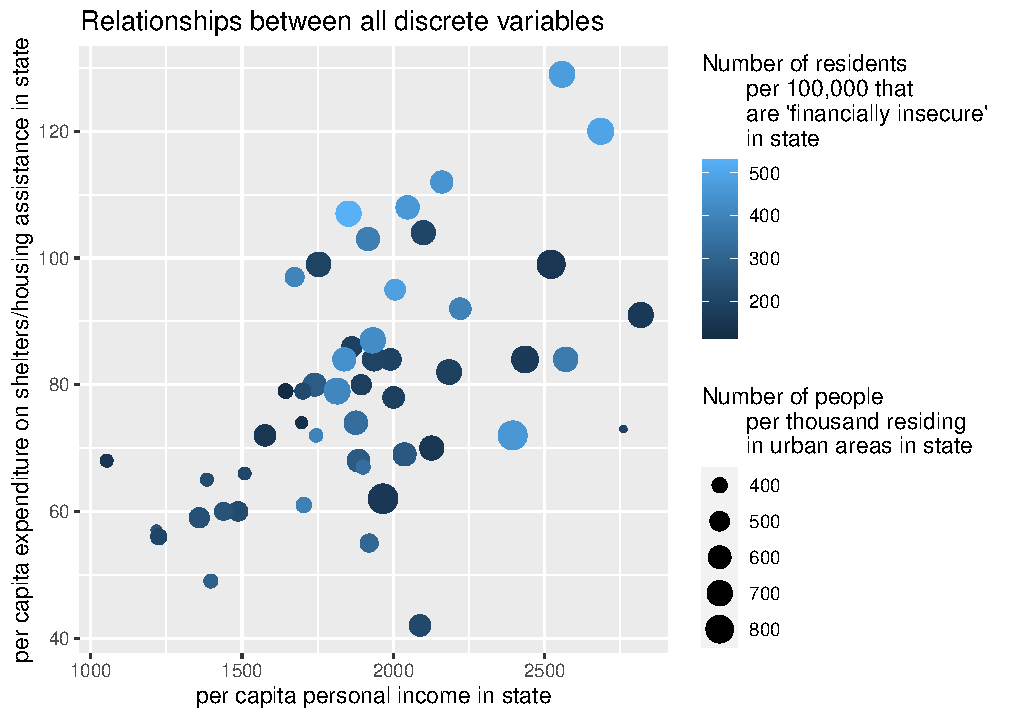
\includegraphics[width=.75\textwidth]{Plot 1.pdf}
\end{figure}

\noindent At a glance, there seems to be a positive correlation between per capita personal income in state, and per capita expenditure on shelter/housing assistance in state, which we can see through the diagonal shape of the axial variables. There does not seem to be any correlation between shelter spending and the other two variables, as the size and colour of the points are vertically distributed fairly randomly. There also appears to be no relationship between the number of financially insecure residents and per capita personal income, as the colour of the points is distributed randomly across the x axis. There does seem to be a positive correlation between per capita personal income and the number of people per capita residing in urban areas, as the size of the points grow along the x-axis.

\end{document}
